% An Applied Mathematics/Biology Thesis
% By Jonathan Niles

\documentclass[phd,tocprelim]{cornell}

% packages
\usepackage{fixltx2e}
\usepackage{geometry}
\usepackage{graphicx}
\usepackage{amsmath,amssymb,amsthm}
\usepackage{tabu}
\usepackage{longtable}
\usepackage{booktabs}
\usepackage{ifpdf}
\usepackage{appendix}
\usepackage[hidelinks]{hyperref}
\usepackage{natbib}
\usepackage[toc]{glossaries}


% cite package, to clean up citations in the main text. Do not remove.
%\usepackage{cite}

% Remove comment for double spacing
%\usepackage{setspace}
%\doublespacing

% Set tolerance for box model
\tolerance=9999

% New Commands, refreshers
%\renewcommand{\caption}[1]{\singlespacing\hangcaption{#1}\normalspacing}
\renewcommand{\topfraction}{0.85}
\renewcommand{\textfraction}{0.1}
\renewcommand{\floatpagefraction}{0.75}

% My own commands
\newtheorem{def}{Definition}
\newcommand{\matr}[1]{\mathbf{#1}}

% Make cornell style
\normalspacing\setcounter{page}{1}\pagenumbering{arabic}
\pagestyle{cornell} \addtolength{\parskip}{0.5\baselineskip}

% LongTabu Fix
\AtBeginEnvironment{longtabu}{\tiny}{}{}   %% change all longtabu content to foot note size

% Make a glossary using the glossaries package
\makeglossaries%

%
% Actual Document Starts here!
%
\begin{document}

% import titlepage
% title.tex

\title{Fragile Architecture in the Human Genome}
\author{Jonathan Niles}
\conferraldate{April}{2015}
\degreefield{Bachelor of Arts}


%\maketitle
%\makecopyright

%\contentspage
%\tablelistpage
%\figurelistpage

% introduction.tex

\chapter{Introduction}

What causes the genome to break?  The human genome is an assemblage of six billion nucleotides encoding the vast instruction set
which controls cell growth, function, and death.  Every possible gene expression pattern is embedded in the genome, yet particular
cell and tissue types arise when the instructions are compiled differently during differentiation.  Some of the great mysteries
of molecular biology surround the establishment and maintenance of the genome structure, and its implications on cell fate. 
Current research indicates the establishment of this \gls{epigenetic} landscape determining cell fate may play an important
role in cancer genesis.

The emerging view of genomic organization indicates that cell regulate expression in local, topologically distinct domains
\citep{guelen2008,dixon2012,pope2014}.  These domains, called topological domains, present a new regulatory agent not
previously described.  Recent work analyzed the architecture \citep{imakaev2012} and epigenetic characteristics
\citep{dixon2012, pope2014}, with implications on gene expression regulation and replication timing.

Topological domains present a novel lens through which to investigate disease, particularly diseases with profound architectural components.
We investigated the structural changes during cell differentiation to establish an architectural link between
nuclear topology and the probability of developing lesions or breaks in the genomic sequence.  We hypothesized that mutations
occurring frequently in specific cancers are based on the epigenetic architecture of the original cell type.  Using human
embryonic stem cells and lung fibroblasts as models, we proposed that topological changes similar to those that establish
patterns of differentiation are responsible for introducing lesions seen in many cell type specific cancers.  To validate our
claim, we applied a heuristic to discover local chromatin topological domains in lung fibroblasts and aligned these domains and
their boundaries to lesions found in the \gls{TCGA}.

This document will proceed as follows.  First, the analytical tools used to perform analysis on genomic data sets are introduced.
These tools include iterative normalization of chromatin contact maps, principal component analysis, and an algorithm to detect
topological domains from contact maps.  A literature review of chromatin architecture is presented to
provide a strong biological intuition regarding chromatin conformation.  Our methods for data acquisition and processing is
described, and we conclude with a discussion of the results and propose areas of further investigation and improvement.

% math.tex

\chapter{Mathematical Preliminaries}

We endeavor to secure a relationship between chromatin topology and genomic fragility to elucidate the progression towards
disease states.  The analytical tools leveraged in the analysis draw from diverse area of mathematics, computational sciences,
and statistics.  We assume the reader has familiarity with the mechanics of linear algebra, an elementary course in statistics,
and numerical analysis.  The reader is heartily encouraged to peruse the references to gain a more complete understanding than
possible to present here.

\section*{Normalization of Chromatin Contact Maps}

The entry point for topological analysis begins with a chromatin \gls{contact map}.  The experimental procedure, called a Hi-C
experiment, generating a chromatin contact map is described in detail in Chapter 3.  For now, we will attempt to motivate our
analysis with a simple thought experiment.

Suppose that one wished to record the conformation of a string, in particular, the loops and intersections where the string crosses
itself or regions lies in close proximity.  One possibility would be to place a one-dimensional coordinate system on the string, say
$0 \geq x \leq  L, x \in \mathbb{N}$.  Regions in close proximity are represented by coordinate pairs $(u,v)$, and we can assemble
them into a graph.  As $L \rightarrow \infty$, the resolution of the matrix increases, and interactions on a smaller scale can be
differentiated.  Figure~\ref{fig:stringmapx} is an example of once such diagram.

\begin{figure}[b]

\end{figure}

The data structure for chromatin modeling is identical in spirit to the model produced in our thought experiment.  However, instead of
interactions occurring on one string, the genome consists of 24 independent chromosome `strings'.  Furthermore, interaction maps are
generated from populations of cells, yielding millions of copies of each genome.  With this in mind, we propose the following definition:

\begin{defn}
  A chromatin contact map $O$ is a symmetric $N \times N$ matrix.  Each cell or bin $O_{ij}$ contains the number of observed contacts
  between regions $i$ and $j$ on the genome.  The contact map is seen as a measure of the \textit{contact probability} between loci
  on a genome-wide scale.
\end{defn}

Contacts are recorded by binning the genome into equally sized intervals and considering the pairwise interactions between each bin.
Typically, bins are ordered by increasing genomic coordinates, from the first bin of chromosome 1 to the last bin of chromosome X.
Depending on data quality, bin sizes range from tens of kilobases to megabases.

The first step of any data analysis pipeline is data \gls{normalization}, which removes experimental biases and noise.  Coupled with quality
control measurements and experimental replicates, normalization also establishes a level of reproducibility.
Several methods exist to normalize contact maps.  Tanay and Yaffe were among the first researchers to undertake a statistical analysis of the
Hi-C experiment in 2011\cite{yaffe2011}.  They identify several sources systematic experimental bias in the Hi-C assay and propose a
probabilistic background model that computes the probability of \glspl{trans contact} and \glspl{cis contact} based on a the regional
\gls{GC} content, fragment length, and genome mappability.  Corrected contact maps are calculated by solving the maximum-likelihood model
parameters on model contact maps, which are then applied to the experimentally derived contact maps.  The mappings
achieved using Tanay and Yaffe's methods provide robust reproducibility between replicates and experiments by considering
\glspl{trans contact} and \glspl{cis contact} separately\cite{yaffe2011}.  However, their analysis pipeline is computationally
intensive, prompting others to research less strenuous methods for Hi-C analysis.

Less computationally intensive methods exist for normalizing contact maps.  Hu and colleagues propose a method `HiCNorm' based on Poisson
regression and achieve a $9000x$ speed up compared to Tanay's method\cite{hu2012}.  Recently, Ay and colleagues provide a statistical method
`Fit-Hi-C' that does not assume a particular underlying statistical distribution, instead normalizing cis contacts based on probabilistic
analysis of polymer looping dynamics\cite{ay2014}.

Imakaev and colleagues propose a normalization and analysis pipeline \gls{ICE}\cite{imakaev2012}.  We employ \gls{ICE} as the normalization
algorithm in this thesis, due to the availability of its source code\footnote{source: \url{http://mirnylab.bitbucket.org/hiclib/}} and good
performance.   We analyze the algorithm in detail.

\subsection*{\glsentryfull{ICE}}

In pursuit of the true contact probability for each genomic region, \gls{ICE} makes a critical observation that bias matrices determined by
Yaffe and Tanay\cite{yaffe2011} can be successfully reproduced ($r = 0.99$) by a product of biases $B_i \times B_j$.  This observation leads
immediately to the following proposition

\begin{prop}
  Given the assumption of factorizable biases, the expected contact frequency $\varepsilon_{ij}$ for every pair of regions $(i,j)$ can
  be written as $\varepsilon_{ij} = B_{i}B_{j}T_{ij}$, where $B_i$ and $B_j$ are biases and $T_{ij}$ is the sought matrix of relative contact
  probabilities, normalized as $\sum_{i, i \neq j, j \pm 1}T_{ij} = 1$.  The normalized contact map is give as
  $T_{ij} = \frac{\varepsilon_{ij}}{B_{i}B_{j}}$.
\end{prop}

The authors note that this normalization procedure results in `equal visibility' regions across the entire genome and maps which are
comparable between Hi-C data sets.  They propose the following algorithm to obtain the biases $B_i$ and `true' relative contact probabilities
$T_{ij}$.

\begin{algorithm}[H]
  \KwData{A matrix of observed interactions $O_{ij}$}
  \KwResult{A matrix of relative contact probabilities $T_{ij}$ and bias vector $B_i$}
  initialize $W^{0}_{ij}$; $B^0 = 1$; $k = 1$\;
  \While{not converged}{%
    $S_i = \sum_{j}W^{k}_{ij}$\;
    $\mean{S_i} = \frac{1}{n}\sum_{i = 1}^{n}S_i$\;
    $\Delta{}B^k_i = \frac{S_i}{\mean{S_i}}$\;
    $W^{k+1}_{ij} = \frac{W^k_{ij}}{\Delta{}B^k_i\Delta{}B^k_j}$\;
    $B^{k+1}_i = B^k_i \dot \Delta{}B^k_i$\;
    \eIf{$\abs{B^{k+1} - B^{k}} < \delta$}{%
      break\;
    }{%
      $k = k + 1$\;
    }
  }
  \caption{Iterative Correction}
\end{algorithm}

It is not apparent that this algorithm is correct or converges.  To gain an intuitive understanding of the solution, let us investigate a
simpler proposition.  Suppose that, instead of defining $O_{ij}$ to be the matrix product $B_{i}B_{j}T_{ij}$, we consider that the counts
in $O_{ij}$ are the expectation of some multinomially distributed random variable $X_{ij}$, where $E[X_{ij}] = NB_{i}B_j$ for some
constant $N$ and vector $B$ whose cumulative sum is 1 ($\sum_{i}B_i = 1$).  In this formulation, we relax our criteria such that each cell
$O_{ij}$ is independent and distributed according to $B$.  The count of cell $i,j$ is given by the probability

\begin{equation}
  p_{ij} = NB_{i}B_{j}
  \log{p_{ij}} =  c + u_i + u_j - Z
\end{equation}

where $c = \log{N}, u_i = \log{B_i}, u_j = \log{B_j}$, and $Z (=c)$ is a normalization factor to ensure that $\sum p = 1$.  This type of
model is called a \gls{log-linear model} or \gls{toric model}.  The problem is now a maximization problem: what are the maximum likelihood parameters
that best fit the model to the observed data?  Luckily, the methods and their convergence properties have been extensively studied in the
literature\cite{fienberg2012, pachter2005}.

In the realm of statistics, the contact matrix, along with the calculated margins, is called a \gls{contingency table}.  Importantly, assuming
that the margins are positive, and that the matrix cannot be permuted into block diagonal shape, Birch's theorem guarantees that there is a
unique maximum to the likelihood function\cite{bishop1975,pachter2005}.  For full details, consult Discrete Multivariate Analysis by
Bishop\cite{bishop1975}.  Furthermore, the marginal values are the \glspl{sufficient statistic} of the model.  In other words, the maximum
likelihood parameters for this data is given by the normalized row and column sums of the matrix\cite{pachter2005}.

With the observation that there exists a global maximum of the likelihood function, all that remains is to compute the `true' values by some
process.  One common algorithm is the \gls{EM} algorithm\cite{fuchs1982}.  Imakaev and colleagues employ a simpler algorithm known as \gls{IPF},
developed by Deming and Stephan in 1940, and apparently rediscovered by Imakaev's group\cite{deming1940}.  \gls{IPF} works generally by solving
the \gls{MLE} while leaving the margins ($p_{i+} = \sum_{j}p_{ij}$ and $p_{j+} = \sum_{i}p_{ij}$) fixed.  A proof of convergence for contingency
tables follows from Fienberg's work in algebraic geometry in 1970\cite{fienberg1970}.

Finally, we return to the \gls{toric model} we described above.  Since the log-likelihood function is concave, the \gls{IPF} algorithm first
computes the roots of the partial derivatives of the log-likelihood function and sets them to zero to solve for the global maximum.  Imakaev
and colleagues consider the likelihood function on the Poisson distribution, given by the \gls{pdf} $f(O;E) = \frac{E^{O}}{O!e^{-E}}$.  The
log-likelihood function for the Poisson distribution is given

\begin{equation}
  LL = \sum_{ij}\left[O_{ij}\log{T_{ij}B_{i}B_{j}} - T_{ij}B_{i}B_{j} - \log{O_{ij}!}\right]
\end{equation}

Differentiating with respect to $T_{lm}$ and $B_m$ and setting the derivatives to zero yields

\begin{multicols}{2}
  \begin{equation}
    \frac{dLL}{d\matr{T}_{lm}} = \frac{O_{lm}}{T_{lm}} - B_{l}B_{m} = 0
    \frac{dLL}{dB_{m}} = \sum_i\left[\frac{\matr{O}_{im}}{B_m} - T_{im}B_i\right] = 0
  \end{equation}

  \break%

  \begin{equation}*
    T_{lm} = \frac{\matr{O}_{lm}}{B_{l}B_{m}}
    \sum_i\left[\frac{\matr{O}_{ij}}{B_{m}B_{i}} - \matr{T}_{im}\right]
  \end{equation}
\end{multicols}

It is clear that the second equation is satisfied if a solution is found for the first.  Taking the first equation with the normalization $T_{ij}$ yields

\begin{equation}
  \sum_i \frac{\matr{O}_{ij}}{B_{i}B_{j}} = 1
\end{equation}

A similar process yields that a broad class of distributions give the same result\cite{imakaev2009}.  \section*{Principal Component Analysis}

The holy grail of data analysis on high-dimensional data is dimensionality reduction --- that is, to find an accurate representation of
the experiment that need not invoke all the dimensions measured.  The benefits of preprocessing the data set into fewer dimensions are
increases in storage capacity and analysis speed.  Since experiments such as Hi-C produce data on larger numbers of features, researchers
attempt to find ways to remove redundancy, eliminate unneeded parameters and compress data sets.  One of the most popular methods is
called \gls{PCA}\cite{law1987}.

Data in high dimensions are difficult to visualize and interpret.  The most common questions in data analysis are `what changed?' or `what
remained the same?' between different experiments.  \gls{PCA} answers these questions by finding a representation of the data that maximizes
the \gls{variance} or variation between observations in the data set.  The output of \gls{PCA} is a transformed data set on a new coordinate
system, called components.  The \glspl{PC} are a subset of these components that capture `most' of the variation in the data set.  It is the
researcher's obligation to compare these components to the original data set and determine what variables or combination thereof, they may
represent.

\begin{defn}[Principal Component Analysis]
  A statistical procedure that transforms a number of possibly correlated variables into a smaller number of uncorrelated variables.
\end{defn}

In practice, there are two methods used for \gls{PCA}.  The simplest to explain, but more error-prone, is the eigen-decomposition
method\cite{smith2006}.  In this procedure, for a data matrix $\matr{A}$, the eigenvalues of the covariance matrix $\matr{A}\matr{A}^T$
are computed directly as the principal components.  However, since this method requires an extra matrix multiplication, numerical
errors are more likely to be introduced during large computations. In practice, \gls{PCA} often derived in conjunction with \gls{SVD}
and we will hold to that standard here.

\begin{thm}[Singular Value Decomposition]
  Let $\matr{A} \in M_{n}(\mathbb{R})$ be given. Then there are unitary matrices $\matr{V} \in M_n$ and $\matr{W} \in M_n$, and a square diagonal
  matrix
  \[
    \matr{\Sigma} =
      \begin{bmatrix}
        \sigma_1 &        & 0        \\
                 & \ddots &          \\
        0        &        & \sigma_n \\
      \end{bmatrix}
  \]
  such that $\sigma_1 \geq \sigma_2 \geq \cdots \geq \sigma_n$ and $\matr{A} = \matr{V}\matr{\Sigma}\matr{W}^*$.  The parameters $\sigma_1$,
  $\hdots$, $\sigma_n$ are the positive square roots of the decreasingly ordered non-zero eigenvalues of $\matr{A}\matr{A}^*$, which are the
  same as the decreasingly ordered nonzero eigenvalues of $\matr{A}^*\matr{A}$.
\end{thm}

To prove that any square matrix $\matr{A} \in M_n(\mathbb{R})$ can be decomposed into singular values, we will use some matrix definitions. The
reader is reminded of the definitions of \textit{normal} $(\matr{A}\matr{A}^* = \matr{A}^*\matr{A})$, \textit{Hermetian} $(\matr{A}^* =  \matr{A})$,
unitary $(\matr{A}^*\matr{A} = \matr{A}\matr{A}^* = 1)$ matrices.  Further, two matrices $\matr{A}, \matr{B} \in M_n$ are said to be
\textit{unitarily similar} they are similar by a unitary matrix $(\matr{A} = \matr{U}\matr{B}\matr{U}^*)$.  Now, we are ready to begin the proof.

\begin{proof}[Singular Value Decomposition]
  It should be clear the matrices $\matr{A}\matr{A}^* \in M_n$ and $\matr{A}^*\matr{A} \in M_n$ have the same eigenvalues, and hence, they are
  unitarily similar.  Then there exists a unitary matrix $\matr{U}$ such that $\matr{A}^*\matr{A} = \matr{U}(\matr{A}\matr{A}^*)\matr{U}^*$.  Then

  \[
    {(\matr{UA})}^*(\matr{UA}) =
    \matr{A}^*\matr{U}^*\matr{UA} =
    \matr{A}^*\matr{A} =
    \matr{UA}\matr{A}^*\matr{U}^* =
    \matr{UA}{(\matr{U}\matr{A})}^*
  \]

  so $\matr{UA}$ is normal.  Let $\lambda_1 = \abs{\lambda_1}e^{i\theta_1}, \ldots, \lambda_n = \abs{\lambda_n}e^{i\theta_n}$ be the positive eigenvalues of
  $\matr{UA}$ in decreasing order.  Furthermore, let $\Delta = diag(\lambda_1, \ldots, \lambda_n)$, let $D = diag(e^{i\theta_1}, \ldots, e^{i\theta_n})$,
  let $\Sigma = diag(\abs{\lambda_1}, \ldots, \abs{\lambda_n})$, and let $\matr{X}$ be a unitary matrix such that $\matr{UA} = \matr{X\Delta}\matr{X}^*$.  Then
  $D$ is unitary and

  \[
    \matr{A} = \matr{U}^*\matr{X}\Sigma\matr{D}\matr{X}^* = (\matr{U}^*\matr{X})\Sigma(\matr{D}\matr{X}^*)
  \]

  If we denote $\matr{V} = \matr{U}^*\matr{X}$ and $\matr{W} = \matr{X}\matr{D}^*$, we have our desired factorization, and
  $\sigma_j = \abs{\lambda_j}, j = 1, \ldots, n$.
\end{proof}

A full proof of \gls{SVD} for rectangular matrices can be found in Horn and Johnson\cite{horn2013}. The relationship between
\gls{SVD} and \gls{PCA} follows directly from the definition of \gls{SVD}.

\begin{thm}
  Let $\matr{A} = \matr{V}\matr{\Sigma}\matr{W}^*$ be the \gls{SVD} of an $n \times n$ dimensional matrix $\matr{A}$ and let

  \[
    \matr{C} = \frac{1}{n - 1}\matr{A}^*\matr{A}
  \]

  be the covariance matrix.  The eigenvectors of $\matr{C}$ are the same as the \textnormal{right singular vectors} of
  $\matr{\Sigma}$.
\end{thm}

\begin{proof}
  Compute
  \[
    \matr{A}^*\matr{A} =
    \matr{V\Sigma}\matr{W}^*\matr{W\Sigma}\matr{V}^* =
    \matr{V\Sigma\Sigma}\matr{V}^* =
    \matr{V}\matr{\Sigma}^2\matr{V}^*
  \]

  \[
    \matr{C} = \matr{V}\frac{\matr{\Sigma}^2}{n - 1}\matr{V}^*
  \]

  $\matr{C}$ is symmetric, and unitarily diagnolizable.  Hence, the eigenvectors of the covariance matrix $\matr{C}$ are the same as the
  matrix $\matr{V}$ (right singular vectors) and the eigenvalues of $\matr{C}$ can be computed directly from the singular values
  $\lambda_i = \frac{\sigma_i}{n - 1}$.
\end{proof}

In principal component analysis, we call the ordered eigenvectors \textit{principal components}.  To ascertain the importance of each
component, one must analyze the \gls{eigenspectrum}, usually in the form of a \gls{scree plot}.  Conceptually, the normalized size of a component's
associated eigenvalue conveys the amount of variation that component captures.  A researcher can the choose a suitable subset of components to
analyze, reducing the dimensionality of the data set the chosen components.

\section*{Detecting changes in local chromatin interaction}

\gls{PCA} is a useful technique for identifying gross differences between data sets.  For subtle changes of local chromatin structure, we appropriate a
technique developed by Bin Ren and colleagues\cite{ren2013}, termed the \gls{DI}.  Intuitively, the \gls{DI} for a given region of chromatin gives the
relative `upstream' or `downstream' character of the interactions involving that particular chromatin region.

The basic premise of the \gls{DI} algorithm is simple.  For each bin along the genome, we calculate the number of upstream and downstream interactions and
assign the normalized difference ($downstream - upstream$) as the \gls{DI} for that particular bin.  The index captures the downstream or upstream bias of
a genomic region. The formulation of the directionality index is given in the supplementary methods of Ren's paper\cite{ren2013}

\[
  DI = (\frac{B - A}{\abs{B - A}})(\frac{{(A - E)}^2}{E} + \frac{{(B - E)}^2}{E})
\]

where $A$ is the number of upstream reads in a given window, $B$ is the number of downstream reads, and $E$ is the expected number of interactions under
the null distribution ($\frac{A + B}{2}$).  Ren and colleagues apply the directionality index to examine 2Mb windows upstream and downstream on a
normalized contact map at 40Kb resolution.

% bio.tex

\chapter{Biological Preliminaries}

\section*{Introduction}

Molecular biology changes daily as new discoveries reinforce or deconstruct previous models of cell function.  The task of
explaining all important aspects of genetics and molecular biology is too large a scope for this thesis; even if we limited
our discussion to simply archetictural interactions.  In the following chapter, we will attempt to cherry-pick topics and recent
developments in genetics and molecular biology to motivate an intuition into chromatin architecture and the potential implications
of a shifting interaction map.  Readers are strongly encouraged to consult a text, such as Molecular Biology of the Cell by
Alberts\cite{alberts2002}, for a more in depth discussion than is possible here.

This chapter begins with a discussion of each actor influencing and influence by nuclear archeticture.  Subsequently, the experiments
to investigate this archeture are introduced, and Hi-C is discussed in detail.  Finally, a theoretical discussion concerning
fragility in the genome presents a backdrop in which to interpret the results of our analytical experiments.


\section*{Building from the Basics}

It is difficult to overstate the importance of chromatin topology.  The morass of nucleic acids and proteins packed tightly inside the
nuclear envelope somehow contains all the information required for cell function and duplication.  The central dogma of molecular biology,
outlined in the notes of Francis Crick `Ideas on Protein Synthesis' in 1956\cite{crick1970} most eloquently illustrates the flow of
information from primary sequence through protein.  At the highest level, the central dogma strongly reinforces the importance of
\gls{DNA} sequence content, readability, and expression.

\begin{figure}[ht]
  % TODO : The central dogma of mol bio
\end{figure}

The sheer complexity of the nucleus is best decomposed into a structural heirarchy with several layers of granularity: the primary
sequence of \gls{DNA} base pairs, architectural modeling proteins, transcription factors and other binding proteins, and \gls{chromosomal
  territories} and other macromolecular chromatin structures.

Ironically, the highest nuclear resolution is the most well studied: the primary sequence of nucleic acid bases that compose the \gls{DNA}
molecule itself.  A single level of abstraction above the primary sequence considers interactions between \gls{DNA} and  architectural
proteins such as histones.  Further up the abstraction heirarchy are \gls{epigenetic} interactions, meaning `above genetics'\cite{dictepi2014},
a loose classification of secondary modifications to \gls{DNA} and architectural proteins that are characteristic of cell type and state.
Finally, chromosomes and chromosomal territories comprise the highest layer of nuclear architecture.  This conceptual heirarchy is useful
to keep in mind when investigating the origin of gene expression changes, differentiation, or disease states.

\subsection*{The Primary Sequence}

The fundamental informational unit of the cell is the \gls{nucleotide}, often called a nucleotide base or base pair when joined in a
molecule or strand.  Eukaryotic cells have a principle four character alphabet of nucleotides, distinguished by their \gls{nucleobases}:
adenine, cytosine, guanine, and thymine.  These nucleotides are affixed to a phosphate backbone in a long, coiling polymer chain.  The
famous publication of the structure of \gls{DNA} in 1953 by researchers James Watson and Francis Crick demonstrated these polymers
exist in the nucleus as double helices\cite{watson1953}.  Hydrogen bonds between opposing nucleotides hold the double helix together.
Importantly, there are two main classifications nucleotides base on structural similarities.  Adenine and guanine are called purine bases,
while thymine and cytosine are called pyridine bases.  Adenine and thymine are complimentary bases that form two hydrogen bonds.  Similarly,
guanine and cytosine are also complementary, and form three hydrogen bonds between their bases.  In this fashion, one strand of the helix completely
determines the opposing side and perturbations from this structure may lead strand mutations\cite{cox2008}.

One cannot ignore the constituents of the primary sequence, particularly when considering macroscopic properties of the genome.  The order and
nucleotide content can change local flexibility and directly (by encoding binding sites) or indirectly (by supporting the binding of histones)
modulates the binding of important architectural proteins\cite{travers2004}.  Although a \gls{DNA} strand is a helical structure, it is an intrinsically
flexible molecule.  A naive calculation reveals that the human genome is roughly two meters in length%
\footnote{%
  A diploid human genome consists of two copies of the $\sim3.1MB$ DNA molecule, based off estimates from the \gls{NCBI} human genome reference build 37.
  Each base pair is assumed to be roughly $0.34\times10^{-9}m$.  The entire length is $2(0.34 \times 10^{-9})(3.2 \times 10^9) = 2.176m$.
},
yet the entire genome fits into a nuclear volume of $\sim523\mu{}m$\cite{marks2011}.  Furthermore, loops as small as 100 bases in length have been
reported in enhancer and repressor element activation pathways\cite{wong2008}. These loops can form independently of proteins\cite{vafabakhsh2012}.
Altogether, \gls{DNA}'s inherent flexibility is the foundation for  many complex higher order chromatin structures.

For completeness, we note that cytosine may undergo methylation, often known as \gls{DNA} methylation or GC methylation to distinguish it
from a histone modification of the same name\cite{bird2002}.  \gls{DNA} methylation is an important epigenetic mark, involved in imprinting,
\gls{X-inactivation}, and heritable epigenetic states\cite{law2010}.  In mammals, \gls{DNA} methylation occurs almost exclusively along
symmetric \gls{GC} dinucleotides, and is estimated to occur at $\sim70-80\%$ of the \gls{GC} sites throughout the genome\cite{ehrlich1982}\cite{law2010}.
In the context of overall chromatin architecture, \gls{DNA} methylation serves a minor role, often reinforcing silencing histone marks; however
one must be cognizant that this repressive mark is a critical regulator local sequence accessibility.

\subsection*{Epigenetics And Chromatin Modeling}

How a \gls{DNA} molecule is packaged and condensed within a cell nucleus remains one of the basic questions of cell biology.  Intellectual curiosity aside,
why is it so important to unravel the chromosomal architecture?  Researcher J.C. Hansen notes, `In biology, structure is inexorably linked to function.'\cite{hansen2012}
The pursuit of an accurate \textit{\gls{in vivo}} model for \gls{DNA} and protein packaging continues to persist today, despite a legacy of experimental,
conceptual, and mathematical models.

In 1974, Kornberg discovered that chromatin contained roughly equal amounts of \gls{DNA} and protein\cite{kornberg1974}.  A year later, Pierre Chambon
and colleagues described the separation of chromatin into protein complexes spaced evenly on the gls{DNA} molecule as `beads on a string.'\cite{oudet1975}
The observed beads are nucleosomes, bundles composed of a histone octamer and $\sim200$ bases (later reported to be $167$ bases\cite{robinson2006}) of
coiled \gls{DNA}. Much as the nucleotide is the fundamental unit of the genome, nucleosomes are the fundamental units of the epigenome.  Nucleosomes in
series are called a \gls{nucleosome array}.  A nucleosome consists of two components: a core particle wrapping $\sim146$ base pairs of DNA, yielding a
6 fold compaction in length, and a linker portion of varying length of $0$ to $\sim80$ base pairs.  The linker component connects adjacent nucleosomes
in a nucleosome array\cite{wu2007}\cite{hansen2012}.  These arrays are $10-nm$ in diameter, provoking them to be often called the `$10-nm$' fibers.

Despite decades of research on nucleosome arrays, their structural conformation \textit{\gls{in vivo}} remains enigmatic.   Does a higher order structure
exist beyond the $10-nm$ fiber?  Nucleosome arrays and linker histones suspended in ionic solution fold naturally into a $30-nm$ fiber\cite{tremethick2007};
however, it is unclear whether this motif forms \textit{\gls{in vivo}} and its conformation may be different in the nuclear context\cite{bian2012}.
The $30-nm$ fiber model is appealing as it readily explains the highly compacted structure of mitotic chromosomes.  To form the fiber, arrays of nucleosomes
are arranged in a solenoid or double-helix structure (for full review, see Grigoryev and Woodcock\cite{grigoryev2012}).  Whether one or both structures
are present in sub-chromosomal architectures is still an open question\cite{song2014}.  Recently, experiments using cryogenic electron microscopy
(cryo-EM) suggested an alternative fractal arrangement of $10-nm$ fibers, without invoking a higher organizational unit\cite{nishino2012}\cite{hansen2012}.
It likely that a mixture of these organizational schemas exist in the cell.  Further research as needed to assess the biological relevance of the $30-nm$ fiber in
both interphase and mitotic chromosome structure.

The nucleosome core particle is a central actor controlling gene expression through local transcription regulation.  It is well established that nucleosomes
cause an attenuation of gene expression when present at physiological concentrations\cite{brown1984}\cite{lorch1987}\cite{laybourn1991}\cite{juan1994}. How
then does the cell maintain some genes as actively transcribed while others are silenced?  Nucleosomes regulate gene expression by regulating accessibility.
Gene expression is mediated by a confluence of protein-DNA interactions: enhancers bind to enhancer elements, polymerases to the transcription start site
(TSS), and polymerase recruitment proteins line the promoter region to facilitate polymerase binding and transcription activation\cite{cox2008}.  At
any protein-DNA junction, local chromatin compaction can exclude binding by physically restricting access to the primary sequence.  This tightly packed
form of DNA is called \textit{\gls{heterochromatin}}, while open and accessible sequence is called \textit{\gls{euchromatin}}.

%%TODO
A critical feature of gene regulation is the ability to form long range
interactions between distal elements of the genome.  Note, cite heintzman et al.

\subsection*{Chromosomes are organized in territories}

The highest level of genome organization is the chromosome territory (CT) or chromosome neighborhood\cite{cremer2001}.
The hypothesis that chromosomes were segregated into nuclear sub-volumes dates back more than 100
years\cite{cremer1993}.  The raison d'etre of these territories is not well understood; however, it is
proposed that CT distribution in the nucleus protects the gene-rich chromosomes by localizing them to
the nuclear center\cite{boyle2001}\cite{federico2006}, CTs create gene expression `pockets' with localized
transcriptional and repair machinery\cite{bolzer2005}, and may have cell type specific positioning.

% TODO Are the chromosomal territories inherited throughout progeny?
% http://ac.els-cdn.com/S0092867403001892/1-s2.0-S0092867403001892-main.pdf?_tid=ccd0bd28-a889-11e4-9e90-00000aab0f26&acdnat=1422627232_949e19f69451fec3a919f3039a1c2a70

To date, there is no evidence to support a deterministic ordering of chromosomes in the nucleus.  However,
there may exist certain deterministic rules to chromosomal positioning.  In all human cell types studied,
the radial position of the chromosomes is correlated with gene density and chromosome size\cite{sun2000}\cite{bolzer2005}.
In most cell types, gene-rich chromosomes are found in the central nuclear compartment, while gene-poor
chromosomes surround the nuclear periphery\cite{boyle2001}\cite{kozubek2005}.  However, in cell types with
non-spherical nuclear shapes, chromosomal arrangements may deviate from this pattern, possibly reflecting
more specialized functions\cite{bolzer2005}.

There is strong evidence that chromosomal territories contain small decondensed regions serving as gene
expression hot-spots.  Unlike bacterial chromosomes, where genes from the same pathway are grouped on the
chromosome in units called \textit{operons}, eukaryotic genes are distributed seemingly randomly throughout
the genome\cite{jacob1961}.  It is well known that transcriptionally active chromatin compartmentalizes based
on replication timing\cite{ferreira1997}\cite{sadoni1999}\cite{thevenin2014}.  Moreover, recent observations
reveal in order to facilitate transcription of genes in a pathway, chromosomal territories co-localize
functionally related genes with transcriptional machinery.  When considering only inter-chromosomal gene pairs,
Thevenin and colleagues observed that co-functioning genes exhibit significant local concentrations, regardless
of linear distance on the primary sequence\cite{thevenin2014}.

% TODO Topologically associated domans?
% http://www.ncbi.nlm.nih.gov/pmc/articles/PMC3874840/

% TODO
% What is this about chromosome neighboorhood location determines translocation outcome?

\chapter{Chromosomal Conformational Capture and Derivatives}

\section*{Capturing Conformations}

The field of molecular biology is advancing rapidly, propelled forth by a
surge of automated techniques.  These so-called `high-throughput' methodologies
enable biologists and bioinformaticians to generate massive data sets with
relative ease, reliability, and efficiency.  The first reference build of the
human genome is a testament to their success\cite{hgsc2004}.  However,
until recently, investigating chromosomal architecture remained an
exhaustively manual process, relying on fluorescence microscopy experiments and
visual inspection by researchers.  It was not until 2003, when Job Dekker and
colleagues described a technique known as Chromosomal Conformational Capture
(3C) that the study of nuclear architecture gained a high throughput methodology
\cite{dekker2002}. Since then, a family of high-throughput capture techniques,
most named a variation on `3C', have been developed to interrogate
different scales and types of chromatin interactions.

The original chromosome conformation capture technique developed by Dekker and
colleagues provides an average measurement of the juxtaposition frequency between
two specific genomic loci in a cell population\cite{frase2014}.  This
interaction frequency measurement is thought to be reflective of the distance
between two associated loci in genomic space.  The first extension of the 3C
experiment, aptly named Chromosome Conformation Capture-on-Chip (4C), increased
the number of interrogated regions from two loci (one to one) to all loci
interacting with a chosen target region (one to all)\cite{simonis2006}.  Most
recently, the Dekker lab extended the method further using biotinylated probes
to assess contacts across the entire genome (all to all)\cite{berkum2010}.
The method, known as Hi-C, boasts the first truly global quantization of every
genomic contact at a given time.

The conceptual idea behind chromosomal conformation capture is remarkably
simple --- to assess nearby regions, the experimenter attempts to fuse
together molecules that are physically close, then determine the interaction
partners of each segment of DNA captured in this fashion.  The 3C procedure
involves five steps.   Initially, a population of cells is cultured in an appropriate
growth medium to a population size of $\sim2.5 \times 10^7$ cells\cite{berkum2010}.
The entire population is treated with formaldehyde, a small chemical commonly
used to fix both cellular samples for microscopy experiments and large specimens
for organismal analysis.  Formaldehyde is a mutagen known to form DNA-DNA and
DNA-protein cross-links\cite{merk1998}.  Importantly, the formaldehyde
treatment covalently binds together proximal DNA and protein structures.
In the second step, the cells are homogenized and chromatin is digested by a
restriction endonuclease, an enzyme that create double-strand cuts at certain
base pair sequences\cite{berkum2010}.  Digestion creates two populations of
DNA fragments: fragments bound to protein/DNA complexes, and an unbound
population.  The unbound population is discarded by filtering.  In the
third step, the bound double-strand sequences are ligated, or joined together,
in highly diluted concentrations. Dilution is critical to ensure ligation
reactions occur only between DNA strands bound to the same molecular complex.
The result of the ligation process is a population of chimeric DNA sequences.
The fourth step reverses the cross-links and release the recombined sequences
from their complexes.  The final step comprises quantifying the restriction
fragments by PCR using primers specific for the population under
study\cite{simonis2007}.

\textbf{TODO}
%
% FIXME
%   The 4C protocol is not very well understood.  Please round out this
% knowledge and fill in the section appropriately.
%

In the derivative methods 4C, 5C, and Hi-C, the basic protocol remains
unchanged; however, the capture and analysis of chimeric fragments varies
depending on the application.  Chromosome Conformation Capture-on-Chip (4C)
leverages a DNA microarray to systematically screen the entire genome in an
unbiased manner for DNA loci that contact a single locus\cite{simonis2006}.
The microarray is tiled with probes which match sequences $< 100$ base pairs
away from a restriction site.  Instead of performing the PCR step from the
canonical 3C assay, restriction fragments are shortened with a second restriction
enzyme, circularized, and amplified by inverse PCR\@.  Amplified probes
are detected by microarray\cite{simonis2006}.  Chromosome Conformation Capture Carbon-Copy (5C)
extends the 3C method by replacing the PCR amplification step with multiplexed
ligation-mediated amplification.  Ligation-mediated amplification (LMA) is a
technique to detect and amplify specific target sequences using primer pairs
that anneal next to each other on the same DNA strand\cite{dostie2006}.
Critically, the 5C method only amplifies strands which are bound by two
primers ligated across the DNA ligation junction, allowing fine control over
the amplified sequences through primer careful design.  Primers are
designed such that forward and reverse 5C primers are ligated across ligation
junctions of select loci in the 3C library.
Furthermore, 5C primers also contain universal tails for amplification,
permitting all bound sequences to be simultaneously amplified.  Thus, through
the appropriate choice of primers, a selected genomic loci is `carbon-copied'
and amplified, allowing high resolution analysis of a given target
interaction\cite{dostie2006}.  The most recent derivation of the technique,
Hi-C, allows comprehensive capture of all interacting segments in the genome
using Next Generation Sequencing (NGS) techniques.  To purify all interacting
segments of the genome, the Hi-C protocol calls for the labeling of all junctions
with biotin markers, effectively marking each genomic junction. Like other
derivative methods, Hi-C abolishes the PCR step of 3C and replaces it with filtration
using streptavidin beads to pull down chimeric DNA sequences.  The captured sequences
can then be sequenced using next generation sequences or hybridized to a
microarray.  More targeted methods ChIA-PET and ChIP-loop incorporate
immunoprecipitation to select complexes containing certain proteins.

\begin{figure}[b]
  \centering
  \caption{An overview of 3C methods.}
  \includegraphics[width=\textwidth]{fig/CompareChromosomeCapture}
  \medskip
  \small
  Chromatin is uniformly cross-linked and digested with a restriction enzyme.
  Bound sequences are immunoprecipitated or biotinylated, depending on the
  assay, and strands are ligated.  Ligation yields novel chimeric sequences
  which are purified.  The number of interactions are assess by qPCR in
  the canonical 3C method and ChIP-loop, inverse PCR in 4C, multiplexed
  sequencing with oligonucleotides in 5C, and paired end sequencing in Hi-C
  and ChIA-PET\@.  Adapted from Montavon \textit{et al.}\cite{montavon2012}.
\end{figure}


\section*{Analysis}

The perceptive reader will note that much can go wrong in a 3C experiment.
Every 3C method involves some level of digestion, ligation, and amplification,
and errors may be introduced at each step.  In particular, Dekker provides
guidelines for three important control steps to ensure the methodology remains
integrous: control of PCR efficiency, determination of background random
collisions and data normalization\cite{dekker2006}.  Many derivative methods
omit the PCR step, however all methodologies must be cognizant that biases are
introduced in any replacement protocol.


Chromosome Conformation Capture is a quantitative assay and meaningful
results are gleaned by comparison of relative interaction frequencies


% TODO
% Combine this chapter and the biology chapter.
\chapter{Fragility in the Code}

The first investigations into nuclear architecture were conducted by
examining cell karyotypes.  Despite the development of the karyotype as a
tool for examining nuclear material in the early 20th
century\cite{levitsky1924}, it wasn't until 1954 the number of chromosomes in
a human cell were definitely described\cite{tjio1956}.  Early investigations
into nuclear architecture, even at the course level of a karyotype, were
hampered by technical limitations and chromosomal phenomena such as
non-dysjunction and breakage.  It is not surprising that soon after the
initial description the human chromosomal number, Debakan and colleagues
characterized common sites were chromosomes would undergo breakage or
translocations.  They termed these regions
\textit{chromosomal fragile sites}\cite{leyden2008}.

Many particularities render studying fragile sites difficult.  The
first difficulty is semantic; chromosomal fragile sites are not precisely
defined in the literature.  When a study is performed that encompasses fragile
sites, typically one of three definitions is used: regions that are particularly
sensitive to forming gaps or breaks on metaphase chromosomes\cite{glover2005},
sites where chromatin fails to compact under mitosis\cite{leyden2008}, and
non-randomly distributed loci that exhibit an increased frequency of breakage
under replicational stress\cite{franchitto2013}.  For the purposes of this
discussion, a \textit{fragile site} is a region on the chromosome prone to
forming complex rearrangements, particularly double-strand breaks, repeat
extensions, and translocations, when subjected to replicational stress.  These
rearrangements play a pivotal role in many severely deliberating genetic
diseases.

Fragile sites come in two flavors: common fragile sites (CFS) and rare fragile
sites (RFS).  Fragile sites are classified into a group based on their
prevalence in the population, and the conditions under which their fragility
is induced\cite{leyden2008}.  Common fragile sites are thought to be common
most chromosomes and to all humans, while rare fragile sites may be expressed
in small fraction (less than 5\%) of the population\cite{wells2006}.

These
rearrangements play pivotal roles in severely debilitating genetic diseases
such as Fragile X Syndrome.  All males and an estimated that 60\% of females
with repeat anomalies near the FRM1 gene on the X chromosome suffer
from severe mental handicap due to these alterations\cite{sutherland1995}.
Additionally, fragile sites are often found rearranged in human
cancers\cite{glover2005}.  Despite these findings, reason fragile site are
fragile is still an unanswered question.

% CFS's may be epigenetically defined. (Molecular profiling of CFS in human fibroblasts
% CFS are conserved based on cell types


% TODO
% Combine this chapter and the biology chapter.
\chapter{Fragility in the Code}

The first investigations into nuclear architecture were conducted by
examining cell karyotypes.  Despite the development of the karyotype as a
tool for examining nuclear material in the early 20th
century\cite{levitsky1924}, it wasn't until 1954 the number of chromosomes in
a human cell were definitely described\cite{tjio1956}.  Early investigations
into nuclear architecture, even at the course level of a karyotype, were
hampered by technical limitations and chromosomal phenomena such as
non-dysjunction and breakage.  It is not surprising that soon after the
initial description the human chromosomal number, Debakan and colleagues
characterized common sites were chromosomes would undergo breakage or
translocations.  They termed these regions
\textit{chromosomal fragile sites}\cite{leyden2008}.

Many particularities render studying fragile sites difficult.  The
first difficulty is semantic; chromosomal fragile sites are not precisely
defined in the literature.  When a study is performed that encompasses fragile
sites, typically one of three definitions is used: regions that are particularly
sensitive to forming gaps or breaks on metaphase chromosomes\cite{glover2005},
sites where chromatin fails to compact under mitosis\cite{leyden2008}, and
non-randomly distributed loci that exhibit an increased frequency of breakage
under replicational stress\cite{franchitto2013}.  For the purposes of this
discussion, a \textit{fragile site} is a region on the chromosome prone to
forming complex rearrangements, particularly double-strand breaks, repeat
extensions, and translocations, when subjected to replicational stress.  These
rearrangements play a pivotal role in many severely deliberating genetic
diseases.

Fragile sites come in two flavors: common fragile sites (CFS) and rare fragile
sites (RFS).  Fragile sites are classified into a group based on their
prevalence in the population, and the conditions under which their fragility
is induced\cite{leyden2008}.  Common fragile sites are thought to be common
most chromosomes and to all humans, while rare fragile sites may be expressed
in small fraction (less than 5\%) of the population\cite{wells2006}.

These
rearrangements play pivotal roles in severely debilitating genetic diseases
such as Fragile X Syndrome.  All males and an estimated that 60\% of females
with repeat anomalies near the FRM1 gene on the X chromosome suffer
from severe mental handicap due to these alterations\cite{sutherland1995}.
Additionally, fragile sites are often found rearranged in human
cancers\cite{glover2005}.  Despite these findings, reason fragile site are
fragile is still an unanswered question.

% CFS's may be epigenetically defined. (Molecular profiling of CFS in human fibroblasts
% CFS are conserved based on cell types

% TODO NOT SURE WHERE THIS GOES

%% Data Validation

%% Iterative Correction and Eigenvalue Expansion

%% Visualization Tools
%% Replication Timing Analysis..?

% results.tex
\chapter{Results}

\section*{Genome Interaction Scaling}
We mapped the reads to the genome as described in the Methods.  Upon mapping reads to interaction matrices, we noted that the number
of observed interactions per bin scales differently by chromosome.  We plotted the percentage of reads observed for each chromosome
in 1Mb bins~\ref{fig:probeScalesMb} and by percentage of chromosome length~\ref{fig:probeScalesPercent}.

\begin{figure}[thp]
  \caption{Chromosome Contacts by Bin}
  \begin{minipage}{0.45\textwidth}%
    \centering
    \caption{}\label{fig:probeScalesMb}
    \includegraphics[width=\textwidth]{./figures/results/probeScalesMb.png}
  \end{minipage}

  \begin{minipage}{0.45\textwidth}
    \centering
    \caption{Contacts by Percent Distance}\label{fig:probeScalesPercent}
    \includegraphics[width=\textwidth]{./figures/results/probeScalesPercent.png}
  \end{minipage}
\end{figure}

% TODO: remark on trans interactions

%We remarked that chromosomes have heterogenous scaling properties.  We examined the character of the chromosome for all replicates
%by computing the x coordinate at which we observed $50\%$ of the total chromosome contacts.  These finding are shown below~\ref{fig:probeCom}.
%
%\begin{figure}
%\end{figure}

\section*{Principal Components and Gene Expression}

We tested whether a change in the compartment character (measured by the principal component) for genomic regions .  Using replicated
IMR90 and hESC gene expression experiments, we plotted the changes in gene expression against the compartment changes, but did not
find any correlation between changes in compartment character and gene expression levels ($\rho = -0.009$, $p$-value negligible.
See Figure~\ref{fig:expressionChangeByCompartment}.)

\begin{figure}[thp]
  \begin{minipage}{0.45\textwidth}%
    \centering
    \caption{Gene Expression Change by Compartment Change}\label{fig:expressionChangeByCompartmentChange}
    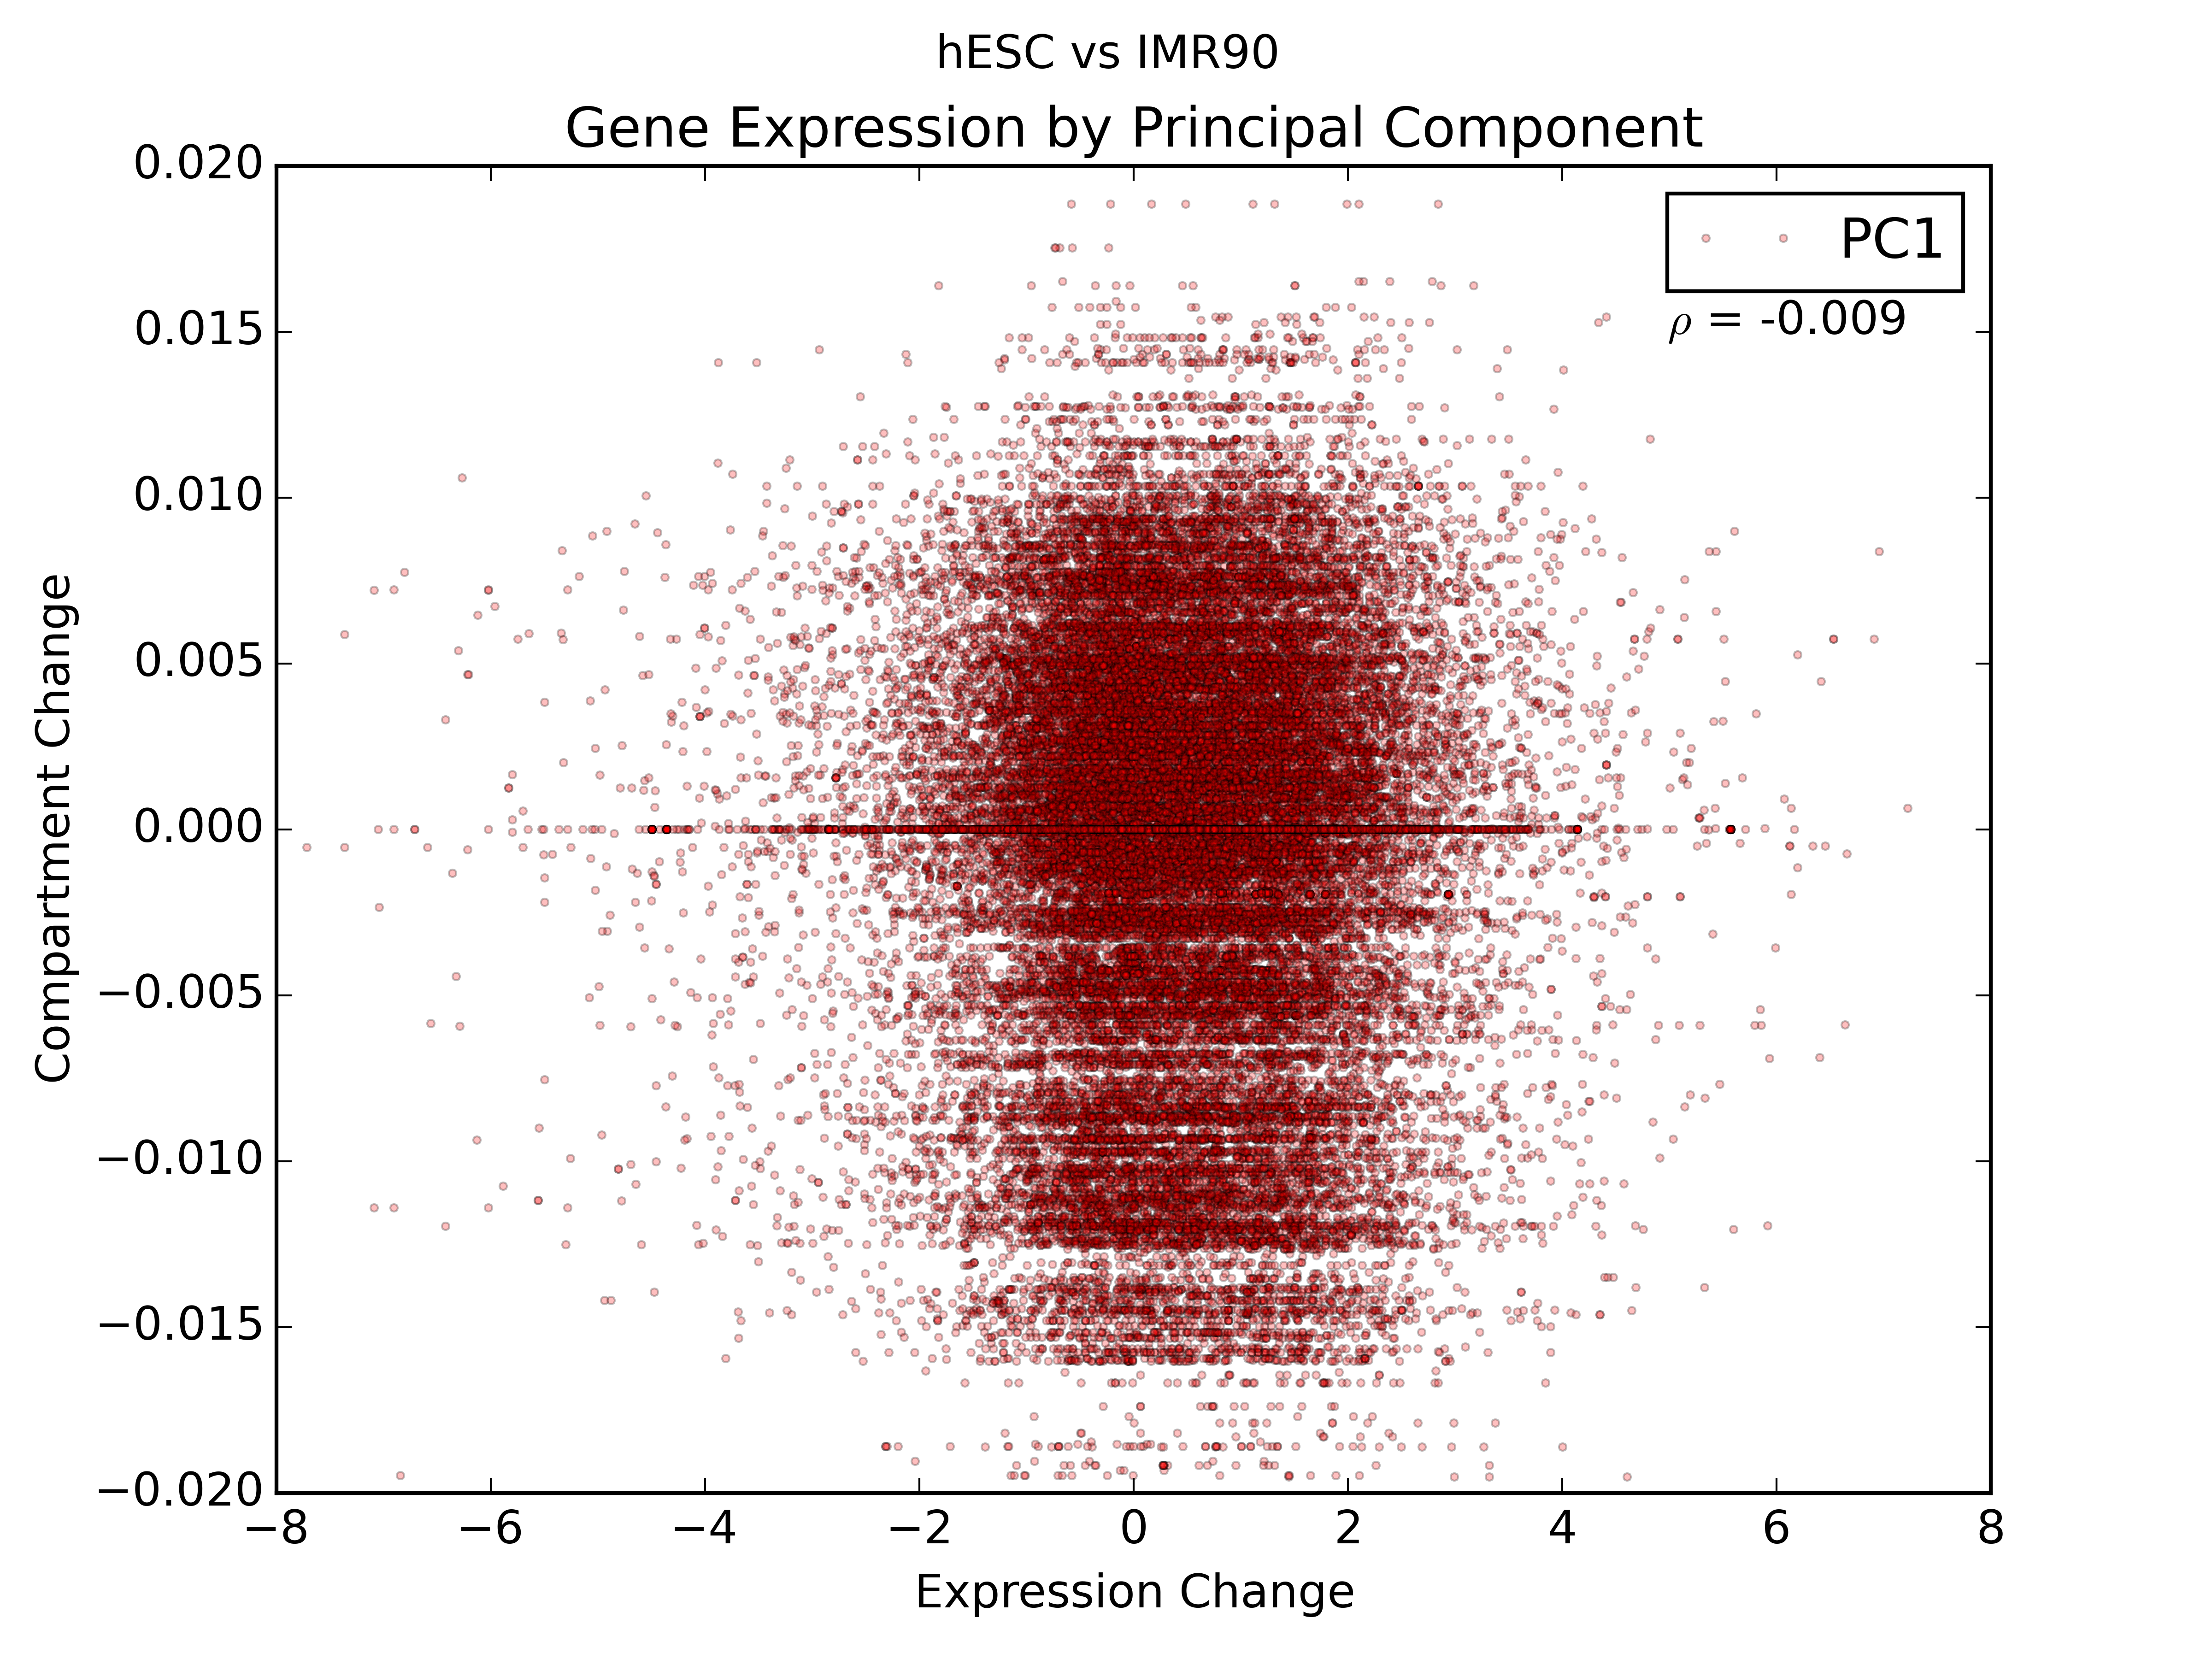
\includegraphics[width=\textwidth]{./figures/results/volcano.png}
  \end{minipage}

  \begin{minipage}{0.45\textwidth}
    \centering
    \caption{Compartmentalized Gene Expression}\label{fig:expressionChangeByCompartment}
    \includegraphics[width=\textwidth]{./figures/results/compartment_ir5_200k.png}
  \end{minipage}
\end{figure}

\section*{Eigenvector Partitioning}

The original Hi-C experiment revealed that the genome can be compartmentalized by \gls{PC} into two characteristic classes, arbitrarily
labeled A and B.  Lieberman-Aiden and colleagues showed positive correlations between compartment identity, gene density, and chromatin
accessibility, concluding that compartment A consists of largely open chromatin, while compartment B is densely packed \citep{aiden2009}.
Interestingly, we did not observe any correlation between the eigenvector and gene expression data (via genome-wide mRNA expression,
Spearman's $\rho = -0.014$, p negligible; Supplementary Information~\ref{}).  Furthermore, shifts in compartment character did not correlate to
changes in gene expression level (Spearman's $\rho = -0.01$, p negligible).  Given these results, it seems unlikely that cells regulate
gene expression at the compartment level.  Compartmentalization appears to be part of the larger nuclear architectural scheme, rather than
a dynamic regulatory mechanism.

Given the known differences between nuclear compartments, we investigated whether common fragile sites were clustered in a particular
compartment, conferring a level of fragility.

\begin{figure}[thp]
  \centering
  \caption{Fragile Sites in Compartments}\label{fig:compartmentCfs}
  \includegraphics[width=\textwidth]{./figures/results/cfs.png}
\end{figure}

\section*{Directionality Indices}

If the nuclear architecture can be decomposed into layers as we have hypothesized, topological domains may exist at different
scales or resolutions within the nucleus.  We tested this hypothesis by calculating directionality indices at various window sizes
on a high resolution contact map.  Interestingly, we found that the minimum correlations between indices at a given window size increased
with higher resolution map ($\rho_{\min}(100kb) = 0.77, \rho_{\min}(1Mb) = 0.70$, Supplementary Information~\ref{sec:SuppDirectionality}).

\section*{Domain Discovery}

Topological domains represent a novel level of genomic regulation.  Previous discovered domains show enrichment in chromatin modeling proteins,
housekeeping genes, and retrotransposons at the topological domain boundaries \citep{dixon2012}.  We used a naive heuristic to discover conserved
topological domain sets at smaller resolutions than previously reported.

\begin{figure}[thp]
  \caption{Number of Domains by Chromosome}
  \begin{minipage}{0.5\textwidth}%
    \centering
    \includegraphics[width=\textwidth]{./figures/results/domain_imr90_bar.png}
  \end{minipage}

  \begin{minipage}{0.5\textwidth}
    \centering
    \includegraphics[width=\textwidth]{./figures/results/domain_hesc_bar.png}
  \end{minipage}
\end{figure}



%
% APPENDIX
%

\appendix
\appendixpage
\addappheadtotoc

% appendix.tex
\chapter{Data Collection}

Methylation data was downloaded from the Salk Institute for Biology Studies in
two files from two biological replicates.  Each file contained $\sim600$ million
reads from the

\begin{table}
  \centering
  \begin{tabular}{lccr}
    \hline
    Replicate & Hg18 Reads & Hg19 Reads & Unlifted Reads \\ \hline
    1 & 563,354,527 & 563,071,323 & 566,408 \\
    2 & 620,520,572 & 620,227,842 & 585,460 \\
    \hline
  \end{tabular}
  \caption{Genomic methylation data for IMR90}
\end{table}

\chapter{Data Migration to Human Genome Build 19}

To make valid comparisons between disparate data sets, it is crucial to ensure all data sets are aligned to the same
build of the human genome.  A genome build is a haploid assembly of sequences from several individuals published by
the NCBI to provide a reference for an organism gene and feature set, though not necessarily every allele.  A build assembly
refers to a particular published sequence annotation set.  Human Genome Build 19 (HG19) is the University of California Santa
Cruz nomenclature for the NCBI Build GRCh37 published in 2009\cite{lander2001}.

In this thesis, the methylation and histone assays were all reported against human genome build 18.  Experiments aligned
against previous builds of the human genome may be updated informatically, either by re-alignment of the
sequence probes or through coordinate transposition.  The UCSC Genome Browser provides a command line utility liftOver for
batch coordinate conversion.  Each file was unzipped and updated to HG19 prior to further analysis using the liftOver tool.

\begin{table}
  \centering
  \begin{tabular}{lccr}
    \hline
    Sample & HG18 Reads & HG19 Reads & Unlifted Reads \\ \hline
    H3K27ac & 16374518 & 16371125 & 3,393 \\
    p65 & 16371125 & 6165230 & 947 \\
    H3K4me1 & 18713234 & 18709033 & 4201 \\
    H3K36me3 & 15808706 & 15807726 & 980 \\
    CTCF & 5501307 & 5499946 & 1361 \\
    \hline
  \end{tabular}
  \caption{Genomic methylation data for IMR90}
\end{table}

\chapter{Iterative Alignment of Probes}

Probes were aligned to the human genome build hg19 using procedures outlined by
Imakaev and colleagues\cite{imakaev2012}.  The chimeric nature of the reads
requires that probes be aligned iteratively, starting from a small, truncated
region from the beginning of the read, mapping this truncated area, increasing
the truncation size and recursing a fixed number of steps or until the alignment
scores become sufficiently poor.  Due to the large number of reads requiring
alignment, we opted to use a fixed truncation length (based on sequence length)
and four steps in the iterative alignment protocol.  The calculation
for the truncation and step size can be found in the the iterativeMapping.py
script provided in the Appendix: Code.  Most reads were 100 base pairs, resulting
in an initial truncation length of 28 base pairs, and step size of 18 base pairs.

Using the mapping functionality from the hiclib python package\cite{imakaev2012},
sequences from the six experimental replicates were realigned to the genome.  The
alignment employed the fast Bowtie2 alignment algorithm\cite{langmead2012}.  Once
aligned, the probes were stored as an interaction matrix in the high performance
HDF5\cite{hdf5} data format, a total of 25Gb for all replicates.

Statistics for iterative alignment are given below:

\begin{center}
  \begin{table}
    \begin{tabular}{l l}
    Total Reads & 2,124,453,478 \\
    Total DS Reads & 1,422,870,270 \\
    Valid Pairs & 713,897,554 \\
    Filtered Reads & 457,298,174 \\
    Percent \textit{trans} Reads & 49.42\% \\
    \end{tabular}
  \end{table}
\end{center}


\chapter{Data Validation}

In order to make meaningful comparisons between data sets (replicates,
in this case), we must show that some degree of relationship exists between
the data sets and comparisons or combinations of the data from disparate sets
are valid to a degree of uncertainty.  It is also essential to understand if the
experimental replicates indeed managed to replicate the conditions of the primary
experiment, or if experimental errors prevent the comparison between replicates.

Spearman's Rank Correlation Coefficient (denoted by the Greek letter $\rho$) is
a non-parametric measure of association between two variables.
Spearman's coefficient assumes some monotonic relationship between variables,
rather than a linear relationship (as in Pearson's), making it appropriate
to compare the IMR90 interaction data sets.  The formula for Spearman's $\rho$ is
given as follows:

\begin{equation}
\rho = 1 - \frac{\sum_{i=1}{n}(d_i^2)}{n(n^2 - 1)}
\end{equation}

where $\rho$ is the correlation coefficient taking values between $-1$ and $+1$,
$d_i = x_i - y_i$ where $x_i, y_i$ are ranks derived from the raw scores $X$ and
$Y$ respectively.

The first replicate IMR90 interaction data set was labeled the primary data set
and the remaining five were compared using Spearman's Rank Correlation.  The
results are given in Table X.

\begin{table}
  \begin{tabular}{|c|*{6}{c|}}
    \toprule
    \textbf{R1} & 0.83 & 0.77 & 0.77 & 0.75 & 0.71 \\ \midrule
    0.83 & \textbf{R2} & 0.82 & 0.83 & 0.79 & 0.75 \\ \midrule
    0.77 & 0.82 & \textbf{R3} & 0.77 & 0.74 & 0.73 \\ \midrule
    0.77 & 0.83 & 0.77 & \textbf{R4} & 0.75 & 0.71 \\ \midrule
    0.75 & 0.79 & 0.74 & 0.74 & \textbf{R5} & 0.69 \\ \midrule
    0.71 & 0.75 & 0.73 & 0.71 & 0.69 & \textbf{R6} \\ \midrule
  \end{tabular}
  \caption{Spearman's $\rho$ across all data sets.}
\label{tab:correlations}
\end{table}


%
% Glossary
%
% Acronym Definitions
\setacronymstyle{long-short}

% Biology
\newacronym{DNA}{DNA}{deoxyribonucleic acid}
\newacronym{RNA}{RNA}{ribonucleic acid}
\newacronym{GEO}{GEO}{Gene Expression Omnibus}
\newacronym{NCBI}{NCBI}{National Center for Biotechnology Information}
\newacronym{SRA}{SRA}{Sequence Read Archive}
\newacronym{TAD}{TAD}{Topologically Associating Domain}
\newacronym{LAD}{LAD}{Lamina Associating Domain}
\newacronym{DS}{DS}{double-stranded}
\newacronym{GC}{GC}{guanine-cytosine}

\newacronym{PCA}{PCA}{Principal Component Analysis}
\newacronym{SVD}{SVD}{Singular Value Decomposition}
\newacronym{PC}{PC}{Principal Component}
\newacronym{ICE}{ICE}{Iterative Correction and Eigenvector Decomposition}
\newacronym{DI}{DI}{Directionality Index}
\newacronym{EM}{EM}{Expectation Maximization}
\newacronym{IPF}{IPF}{Iterative Proportional Fitting}
\newacronym{MLE}{MLE}{Maximum Likelihood Estimation}

% Glossary definitions
\newglossaryentry{karyotype}{%
  name={karyotype},
  description={A photomicrograph of chromosomes arranged according to a standard classification}%
}

\newglossaryentry{trans contacts}{%
  name={trans contacts},
  description={Interactions that occur between bins on two different chromosomes}%
}

\newglossaryentry{cis contacts}{%
  name={cis contacts},
  description={Interactions that occur between bins on the same chromosome}%
}

\newglossaryentry{contact map}{%
  name={contact map},
  description={A non-negative, square matrix recording observed interactions between different genomic regions}%
}

\newglossaryentry{polymer}{%
  name={polymer},
  description={A substance that has a molecular structure consisting chiefly or entirely of a large number of similar units bonded together, e.g., many synthetic organic materials used as plastics and resins}
}

\newglossaryentry{epigenetic}{%
  name={epigenetic},
  description={Any heritable influence on gene activity, unaccompanied by a change in the DNA}
}

\newglossaryentry{restriction enzyme}{%
  name={restriction enzyme},
  description={An enzyme that restricts, or performs double-strand cut, at a specific DNA sequence motif}
}

\newglossaryentry{ligation}{%
  name={ligation},
  description={The joining of two DNA strands or other molecules by a phosphate ester linkage}
}

\newglossaryentry{oligonucleotide}{%
  name={oligonucleotide},
  description={A polynucleotide whose molecules contain a relatively small number of nucleotides}
}

\newglossaryentry{nucleosome}{%
  name={nucleosome},
  description={A chromatin secondary structure consisting of $\sim147$ base pairs of DNA wrapped 1.75 times around an octamer of core histone proteins}
}

\newglossaryentry{scree plot}{%
  name={scree plot},
  description={A graph displaying the eigenvalue associated with each component in descending order versus the component number.  Used in PCA to determine how many components to consider in the analysis}
}

\newglossaryentry{eigenspectrum}{%
  name={eigenspectrum},
  description={A spectrum of eigenvalues}
}

\newglossaryentry{normalization}{%
  name={normalization},
  description={An attempt to compensate for noise and systematic bias from in a particular data set, while preserving the differences in a data set}
}

\newglossaryentry{toric model}{%
  name={toric},
  description={A background model for a distribution.  Also known as a log-linear model}
}

\newglossaryentry{log-linear model}{%
  name={log-linear model},
  description={See toric model.}
}

\newglossaryentry{transcriptome}{%
  name={transcriptome},
  description={The sum total of all messenger RNA molecules expressed from genes of an organism}
}

\newglossaryentry{contingency table}{%
  name={contingency table},
  description={A type of table in statistics that displays the frequency distribution of variables.  Also called a crosstab}
}

\newglossaryentry{sufficient statistic}{%
  name={sufficient statistic},
  description={A statistic that does as good a job estimating an unknown parameter as the entire sample}
}

\newglossaryentry{norm}{%
  name={norm},
  description={In linear algebra, a norm is a function that assigns a strictly non-negative length to each vector in a vector space}
}


%
% BIBLIOGRAPHY
%

\bibliography{bibliography}{}
\bibliographystyle{plos2015}

\printglossaries

\end{document}
